\label{tag:LTI}
LTI(Learning Tools IterOperability)とは、異なるプラットフォーム間における学習支援ツールの相互運用を可能にするための規格[3]であり、ツール間の通信プロトコルはHTTP上でのメッセージ交換として実装されている。\\
LTIに準拠することの具体的なイメージとして、次のケースを想定することができる

\begin{figure}[htbp]
  \begin{center}
    \resizebox{\textwidth}{!}{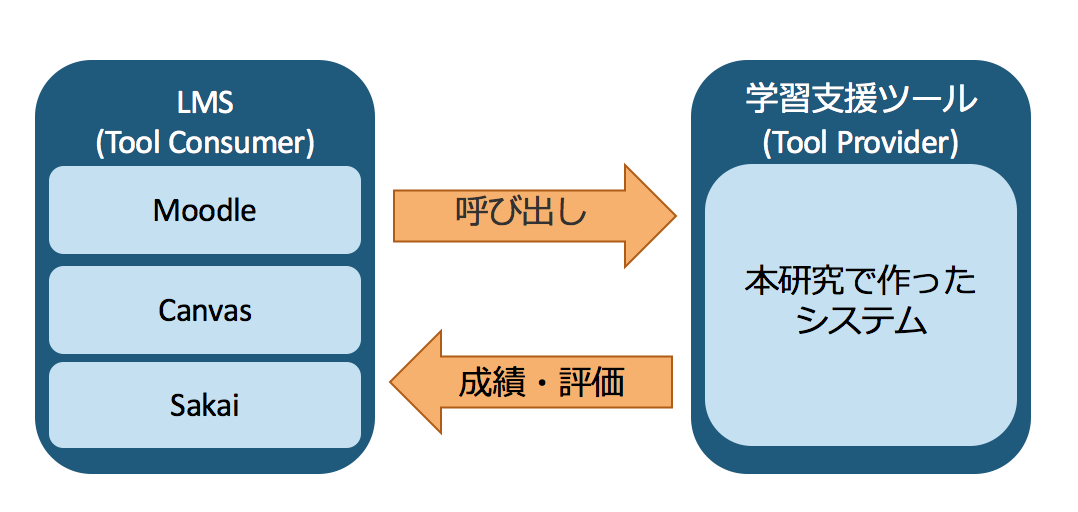
\includegraphics{img/LTIgaiyou.png}}
    %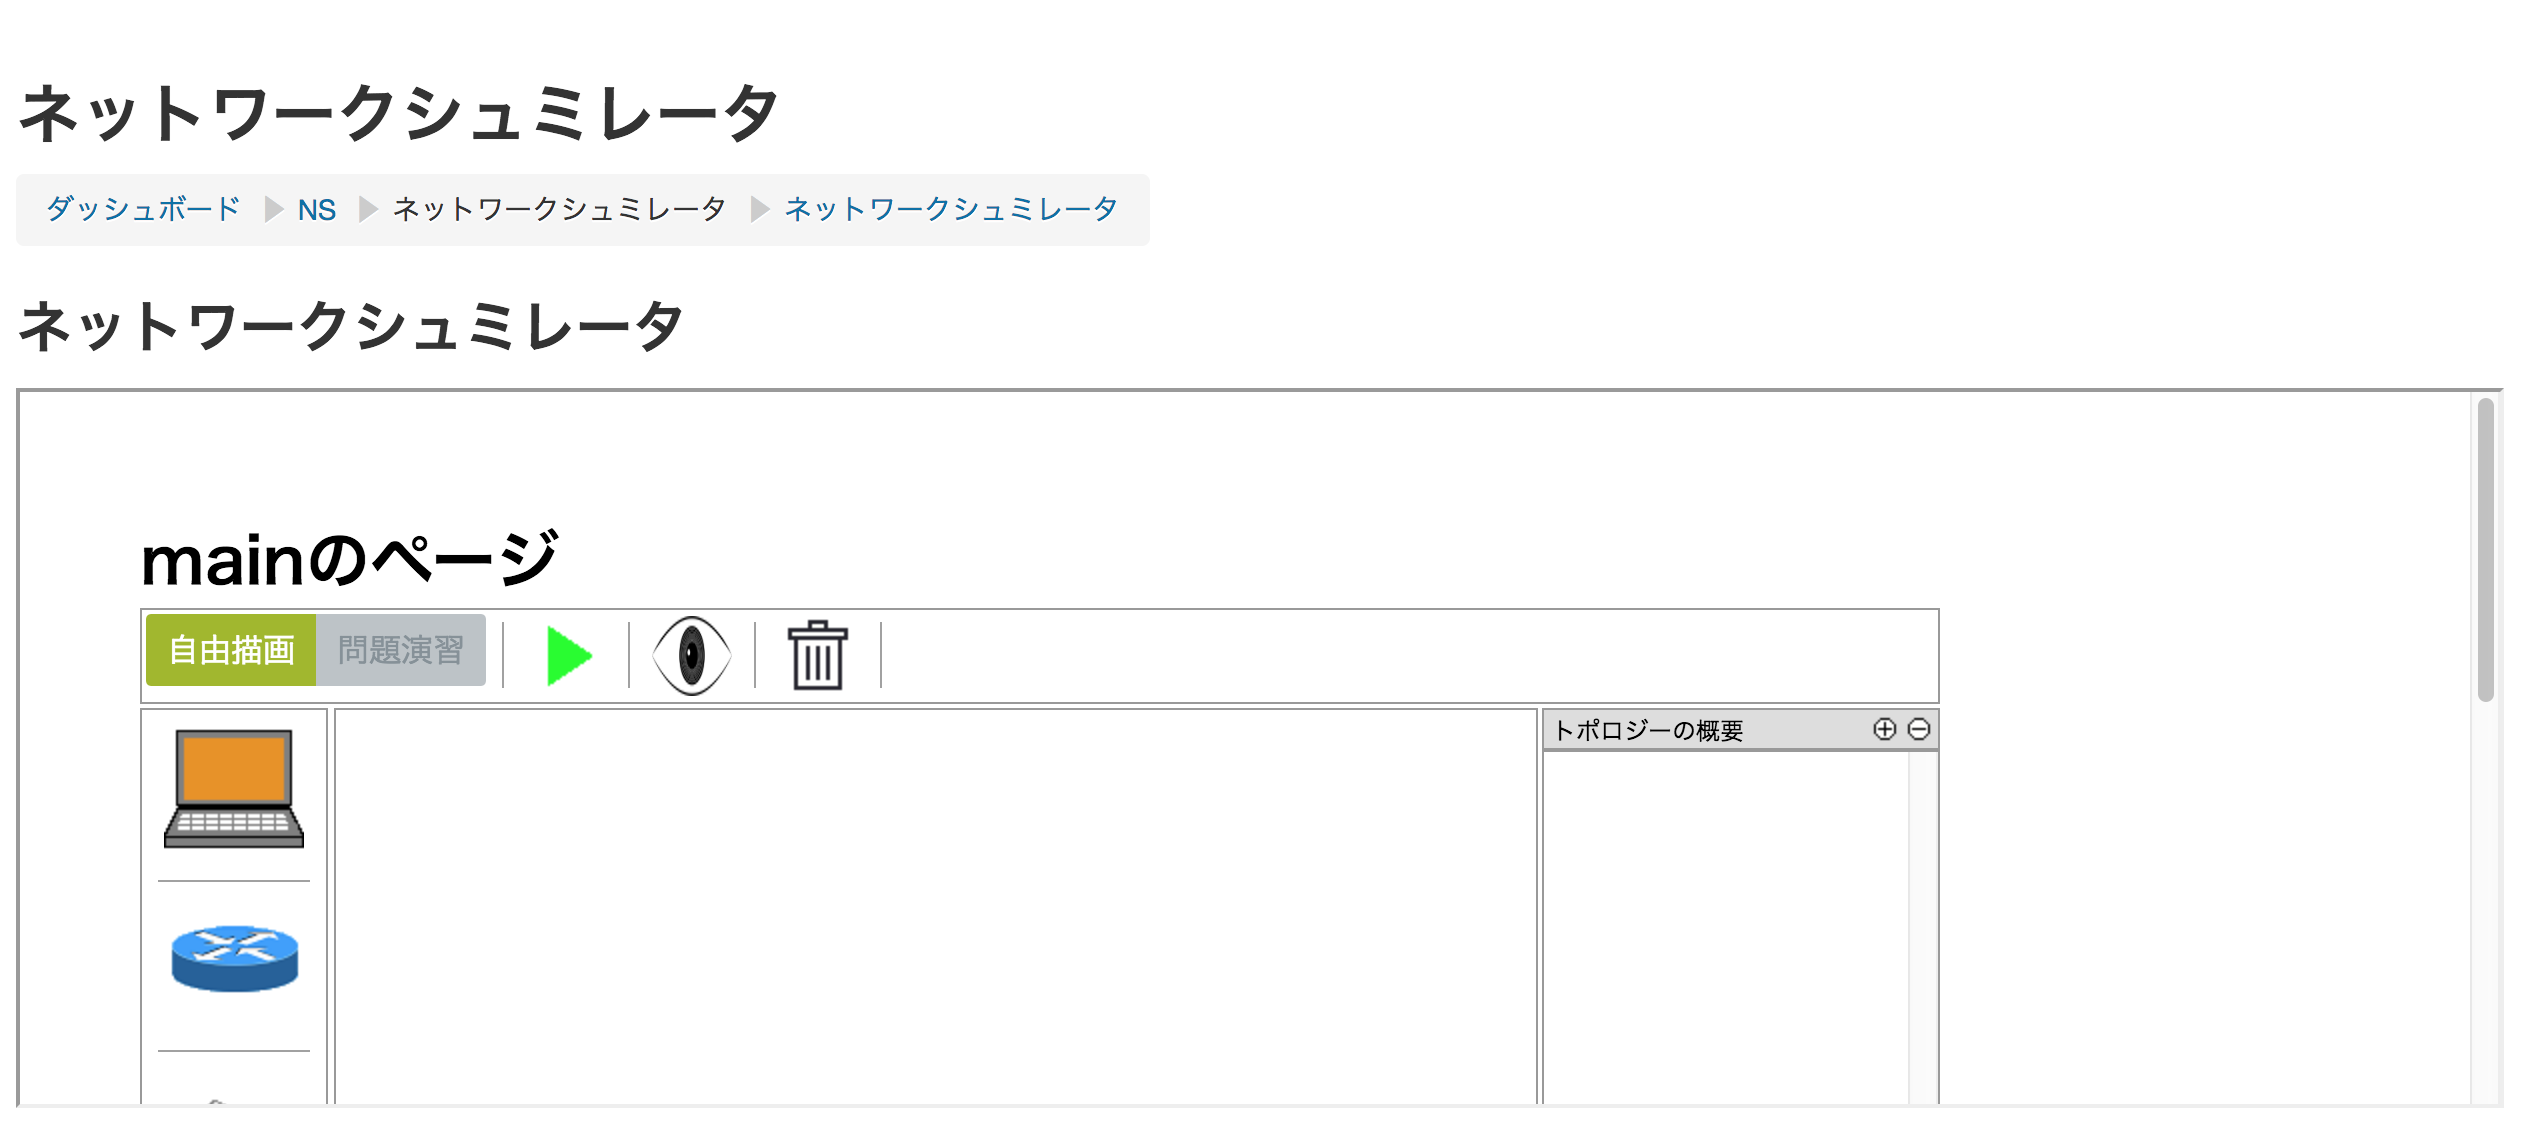
\includegraphics[clip,width=12.0cm,height=8.0cm]{img/LTIstart.png}
    \caption{LTI具体的なイメージ}
    \label{fig:LTI gaiyou}
  \end{center}
\end{figure}

LTIでは、ユーザ情報や課題の進行状況を直接管理するLMSをツールコンシューマと呼ぶ。
標準機能としてLTIに対応しているLMSとして、Canvas, Moodle, Sakai, Blackboardなどがある。
一方、個別の具体的な問題や教材を提供するプラットフォームをツールプロバイダと呼ぶ。LTIに準拠したツールプロバイダを実装すれば、LTIに対応した複数のLMSからツールを実行することが可能となる。
これはツールをプラグインとして実装するのに比べてソフトウェア開発効率の面で極めて有利である。\\

ユーザーとツールコンシューマ間では、ユーザーIDとPWを用いて認証を行う。しかし、ユーザーがツールコンシューマでツールプロバイダを使用する際は、IDとPWを再度入力せずに使用することができ、ユーザーからはLMSの機能の一部かのようにして見える。
これがLTIの利点であり、この認証を省くためにOAuthと呼ばれるプロトコルが使われている。
\subsection{OAuth}
OAuth(オーオース)とは、SNSやWebサービス間で「アクセス権限の認可」を行うためのプロトコルである。また、OAuthには1.0と2.0が存在しているが、本研究ではLTI1.0の実装にあたりOAuth1.0を使用している。
\subsection{LTI1.0におけるOAuth1.0}
OAuth1.0実装では、第三者による不正なログインを防ぐためのOAuth signature(署名)及びkey(暗号)の作成をする必要があった。
しかし、現在OAuth2.0が主流の中、LTI1.0ではOAuth1.0が採用されているため、署名および暗号を作成する関数をRubyで自作した。\\
署名及び暗号の作成手順を以下に示す。\\
1.「キー」を作成\\
2.「文字列」の作成\\
3.「キー」と「文字列」用いて署名を作成\\
\subsubsection{キーの作成}
「oauth\_consumer\_secret」、「oauth\_token\_secret」をRFC 3986に基づきURLエンコードし、&で繋げれば完成。\\
本研究では「oauth\_consumer\_secret」を設定し、「oauth\_token\_secret」は存在させなかった。また、各々をRFC 3986に基づきURLエンコードし、「oauth token secret」を空白とし、\&のみを繋げてKeyを作成した。
\subsubsection{文字列の作成}
1.パラメータをアルファベット順に並べ、キー=値...の形で並べた上で,RFC 3986に基づきURLエンコードする。\\
2.リクエストメソッド、リクエストURLをRFC 3986に基づきURLエンコードする。\\
3.リクエストメソッド、リクエストURL、パラメータの順で\&で繋げることで文字列を作成した。\\
\subsubsection{署名の作成}
1.LTI1.0ではHMAC-SHA1方式を採用しているため、作成した「キー」と「署名」を用いてHMAC-SHA1方式でハッシュ値を生成する。この時バイナリデータでハッシュ値を生成する必要がある。\\
2.生成したハッシュ値を、base64エンコードすることで作成。この手順で出てきた数値が署名となる。\\
\subsection{成績反映}
成績反映の手順を以下に示す。\\
ツールコンシューマから成績を返すパラメータ「lis\_outcome\_service\_url」を設定し、特定のユーザーを一意的に示す、「SourcedId」をパラメータ「lis\_result\_sourcedid」から取得し、XML内の「SourcedId」を書き変え、ツールプロバイダでまとめた点数をXML内の「textString」に加えた上で送信する。\\
